La implementación de las fuentes de tensión de \SI{12}{\volt} y \SI{-12}{\volt} se realizó en base a los circuitos integrados \texttt{LM2576} y \texttt{LM2577}. Se propuso la construcción de dos circuitos independinetes, con el fin de no consumir toda la corriente de una sola fuente.

\subsection{Fuente reductora de tensión}
El diseño propuesto en la Figura \ref{fig.fte_12} corresponde a la configuración reductora de tensión cuya entrada es \SI{+30}{\volt}, y su salida \SI{+12}{\volt}. Debido a la dificultad de conseguir el modelo \textit{LM2565-12}, se decidió utilizar la versión ajustable, la cuál implica anexar dos resistencias de realimentación $R_2$ y $R_3$ según el esquema. El inductor $L_2$ y el capacitor $C_3$ permiten reducir el riple de la tensión de salida.


%\begin{figure}[H]
	%\centering
%	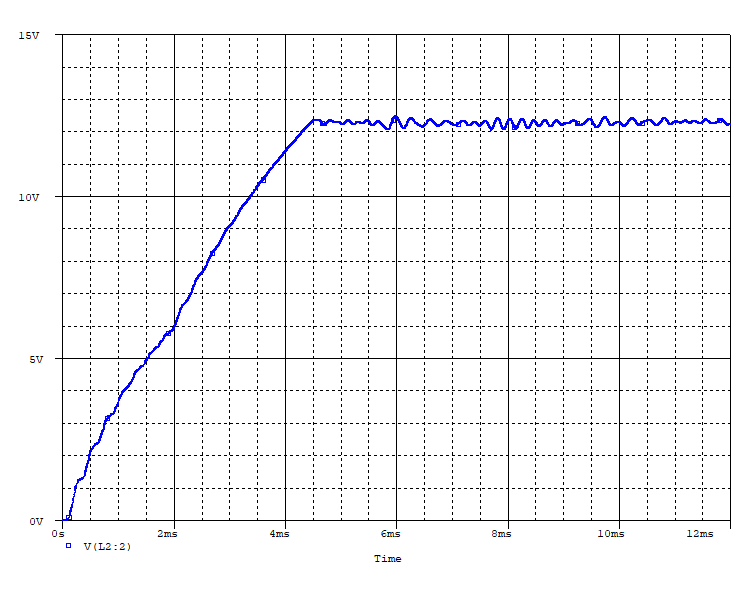
\includegraphics[angle=-90,width=1.1\textwidth, trim = 0.5cm 3.0cm 4cm 4cm]{fte_12_salida.png}
%	\caption{Salida de la fuente reductora de tensión.}
%	\label{fig.fte_salida_12}
%\end{figure}


\begin{figure}
	\centering
	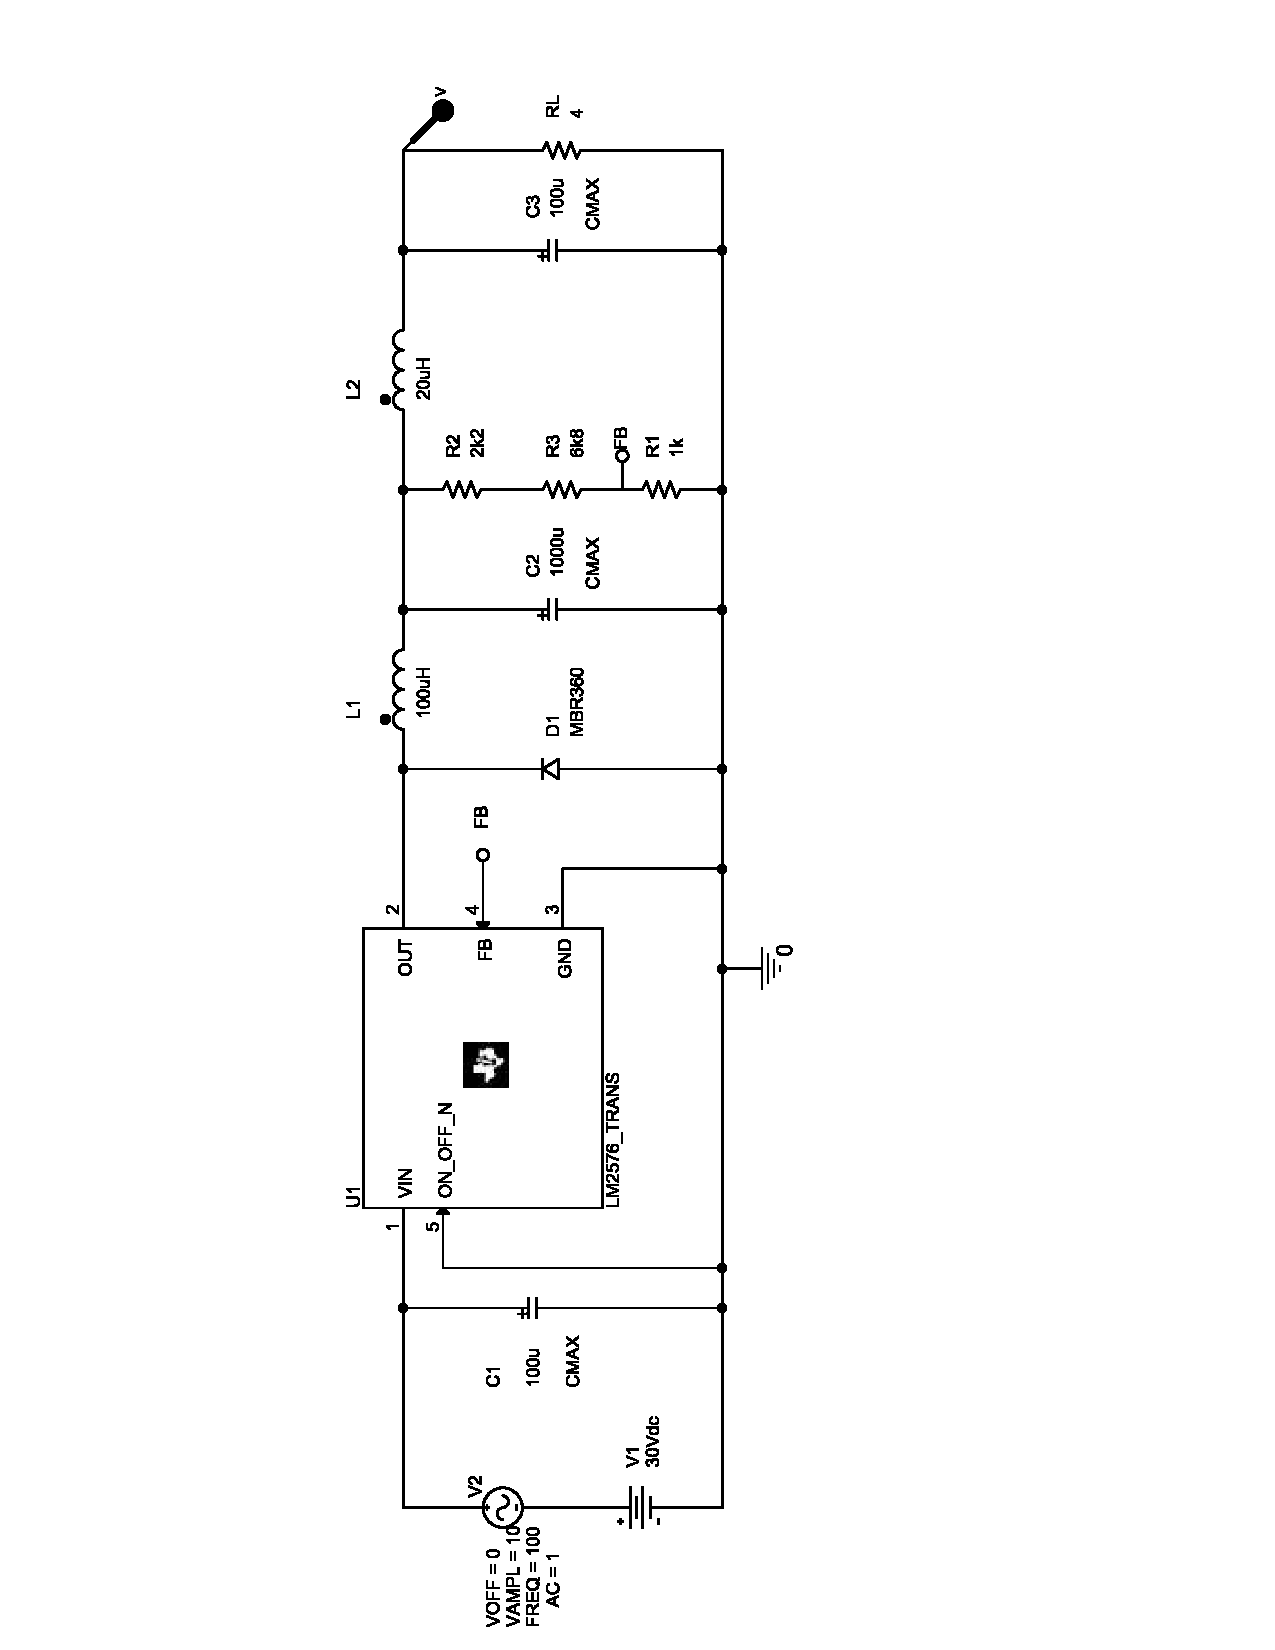
\includegraphics[width=0.4\textwidth, angle=-90, trim= 4.0cm 3cm 7cm 4cm]{fte_12_esquema.pdf}
	\caption{Fuente reductora de tensión.}
	\label{fig.fte_12}
\end{figure}


Debido a que la fuente de entrada puede variar en un 20\%, en la simulación se anexó una fuente alterna en serie para analizar el comportamiento de la salida ante alteraciones de $V_E$. La salida resultante se muetra en la Figura \ref{fig.fte_salida_12}, observándose una variación del orden de decenas de $\SI{}{\milli\volt}$.



\HgraficarPNG{0.5}{fte_12_salida}{Salida de la fuente reductora de tensión}{fig.fte_salida_12}


\subsection{Fuente elevadora de tensión}

Para el circuito elevador, desde \SI{-30}{\volt} a \SI{-12}{\volt}, se propuso el diseño de la Figura \ref{fig.fte_elevadora}. 
No se logró realizar la simulación debido a la inexistencia del modelo de \texttt{LM2577} en \emph{PSpice}. 
La elección de los componentes se detalla en la nota de aplicación, aunque sus valores podrán variar empíricamente.

\begin{figure}[H]
	\centering
	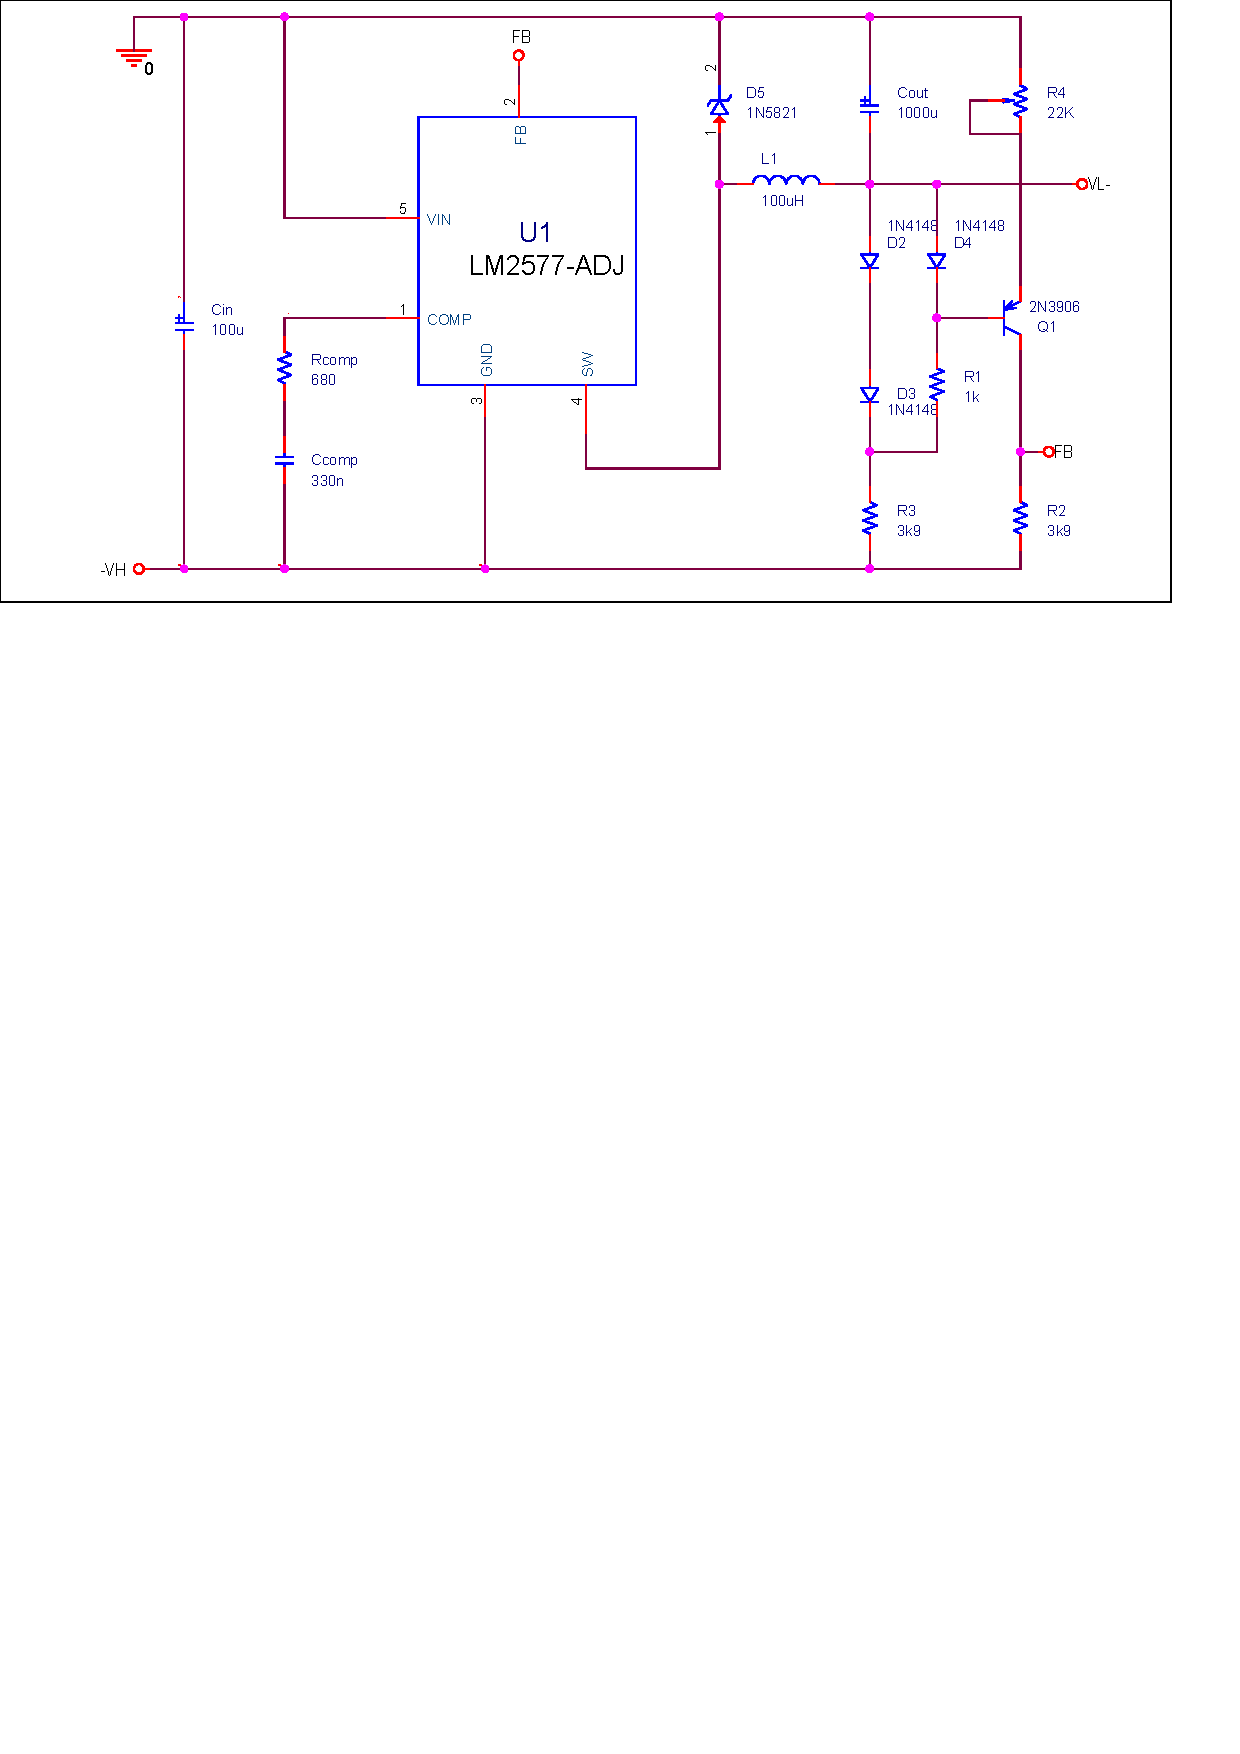
\includegraphics[width=0.6\textwidth, trim = 0cm 19cm 2cm 0cm]{lm2577}
	\caption{Fuente elevadora de tensión.}
	\label{fig.fte_elevadora}
\end{figure}

